% Options for packages loaded elsewhere
\PassOptionsToPackage{unicode}{hyperref}
\PassOptionsToPackage{hyphens}{url}
%
\documentclass[
]{article}
\usepackage{amsmath,amssymb}
\usepackage{lmodern}
\usepackage{ifxetex,ifluatex}
\ifnum 0\ifxetex 1\fi\ifluatex 1\fi=0 % if pdftex
  \usepackage[T1]{fontenc}
  \usepackage[utf8]{inputenc}
  \usepackage{textcomp} % provide euro and other symbols
\else % if luatex or xetex
  \usepackage{unicode-math}
  \defaultfontfeatures{Scale=MatchLowercase}
  \defaultfontfeatures[\rmfamily]{Ligatures=TeX,Scale=1}
\fi
% Use upquote if available, for straight quotes in verbatim environments
\IfFileExists{upquote.sty}{\usepackage{upquote}}{}
\IfFileExists{microtype.sty}{% use microtype if available
  \usepackage[]{microtype}
  \UseMicrotypeSet[protrusion]{basicmath} % disable protrusion for tt fonts
}{}
\makeatletter
\@ifundefined{KOMAClassName}{% if non-KOMA class
  \IfFileExists{parskip.sty}{%
    \usepackage{parskip}
  }{% else
    \setlength{\parindent}{0pt}
    \setlength{\parskip}{6pt plus 2pt minus 1pt}}
}{% if KOMA class
  \KOMAoptions{parskip=half}}
\makeatother
\usepackage{xcolor}
\IfFileExists{xurl.sty}{\usepackage{xurl}}{} % add URL line breaks if available
\IfFileExists{bookmark.sty}{\usepackage{bookmark}}{\usepackage{hyperref}}
\hypersetup{
  pdftitle={Important Penguin Analysis},
  hidelinks,
  pdfcreator={LaTeX via pandoc}}
\urlstyle{same} % disable monospaced font for URLs
\usepackage[margin=1in]{geometry}
\usepackage{color}
\usepackage{fancyvrb}
\newcommand{\VerbBar}{|}
\newcommand{\VERB}{\Verb[commandchars=\\\{\}]}
\DefineVerbatimEnvironment{Highlighting}{Verbatim}{commandchars=\\\{\}}
% Add ',fontsize=\small' for more characters per line
\usepackage{framed}
\definecolor{shadecolor}{RGB}{248,248,248}
\newenvironment{Shaded}{\begin{snugshade}}{\end{snugshade}}
\newcommand{\AlertTok}[1]{\textcolor[rgb]{0.94,0.16,0.16}{#1}}
\newcommand{\AnnotationTok}[1]{\textcolor[rgb]{0.56,0.35,0.01}{\textbf{\textit{#1}}}}
\newcommand{\AttributeTok}[1]{\textcolor[rgb]{0.77,0.63,0.00}{#1}}
\newcommand{\BaseNTok}[1]{\textcolor[rgb]{0.00,0.00,0.81}{#1}}
\newcommand{\BuiltInTok}[1]{#1}
\newcommand{\CharTok}[1]{\textcolor[rgb]{0.31,0.60,0.02}{#1}}
\newcommand{\CommentTok}[1]{\textcolor[rgb]{0.56,0.35,0.01}{\textit{#1}}}
\newcommand{\CommentVarTok}[1]{\textcolor[rgb]{0.56,0.35,0.01}{\textbf{\textit{#1}}}}
\newcommand{\ConstantTok}[1]{\textcolor[rgb]{0.00,0.00,0.00}{#1}}
\newcommand{\ControlFlowTok}[1]{\textcolor[rgb]{0.13,0.29,0.53}{\textbf{#1}}}
\newcommand{\DataTypeTok}[1]{\textcolor[rgb]{0.13,0.29,0.53}{#1}}
\newcommand{\DecValTok}[1]{\textcolor[rgb]{0.00,0.00,0.81}{#1}}
\newcommand{\DocumentationTok}[1]{\textcolor[rgb]{0.56,0.35,0.01}{\textbf{\textit{#1}}}}
\newcommand{\ErrorTok}[1]{\textcolor[rgb]{0.64,0.00,0.00}{\textbf{#1}}}
\newcommand{\ExtensionTok}[1]{#1}
\newcommand{\FloatTok}[1]{\textcolor[rgb]{0.00,0.00,0.81}{#1}}
\newcommand{\FunctionTok}[1]{\textcolor[rgb]{0.00,0.00,0.00}{#1}}
\newcommand{\ImportTok}[1]{#1}
\newcommand{\InformationTok}[1]{\textcolor[rgb]{0.56,0.35,0.01}{\textbf{\textit{#1}}}}
\newcommand{\KeywordTok}[1]{\textcolor[rgb]{0.13,0.29,0.53}{\textbf{#1}}}
\newcommand{\NormalTok}[1]{#1}
\newcommand{\OperatorTok}[1]{\textcolor[rgb]{0.81,0.36,0.00}{\textbf{#1}}}
\newcommand{\OtherTok}[1]{\textcolor[rgb]{0.56,0.35,0.01}{#1}}
\newcommand{\PreprocessorTok}[1]{\textcolor[rgb]{0.56,0.35,0.01}{\textit{#1}}}
\newcommand{\RegionMarkerTok}[1]{#1}
\newcommand{\SpecialCharTok}[1]{\textcolor[rgb]{0.00,0.00,0.00}{#1}}
\newcommand{\SpecialStringTok}[1]{\textcolor[rgb]{0.31,0.60,0.02}{#1}}
\newcommand{\StringTok}[1]{\textcolor[rgb]{0.31,0.60,0.02}{#1}}
\newcommand{\VariableTok}[1]{\textcolor[rgb]{0.00,0.00,0.00}{#1}}
\newcommand{\VerbatimStringTok}[1]{\textcolor[rgb]{0.31,0.60,0.02}{#1}}
\newcommand{\WarningTok}[1]{\textcolor[rgb]{0.56,0.35,0.01}{\textbf{\textit{#1}}}}
\usepackage{graphicx}
\makeatletter
\def\maxwidth{\ifdim\Gin@nat@width>\linewidth\linewidth\else\Gin@nat@width\fi}
\def\maxheight{\ifdim\Gin@nat@height>\textheight\textheight\else\Gin@nat@height\fi}
\makeatother
% Scale images if necessary, so that they will not overflow the page
% margins by default, and it is still possible to overwrite the defaults
% using explicit options in \includegraphics[width, height, ...]{}
\setkeys{Gin}{width=\maxwidth,height=\maxheight,keepaspectratio}
% Set default figure placement to htbp
\makeatletter
\def\fps@figure{htbp}
\makeatother
\setlength{\emergencystretch}{3em} % prevent overfull lines
\providecommand{\tightlist}{%
  \setlength{\itemsep}{0pt}\setlength{\parskip}{0pt}}
\setcounter{secnumdepth}{-\maxdimen} % remove section numbering
\ifluatex
  \usepackage{selnolig}  % disable illegal ligatures
\fi

\title{Important Penguin Analysis}
\author{}
\date{\vspace{-2.5em}}

\begin{document}
\maketitle

\begin{figure}
\centering
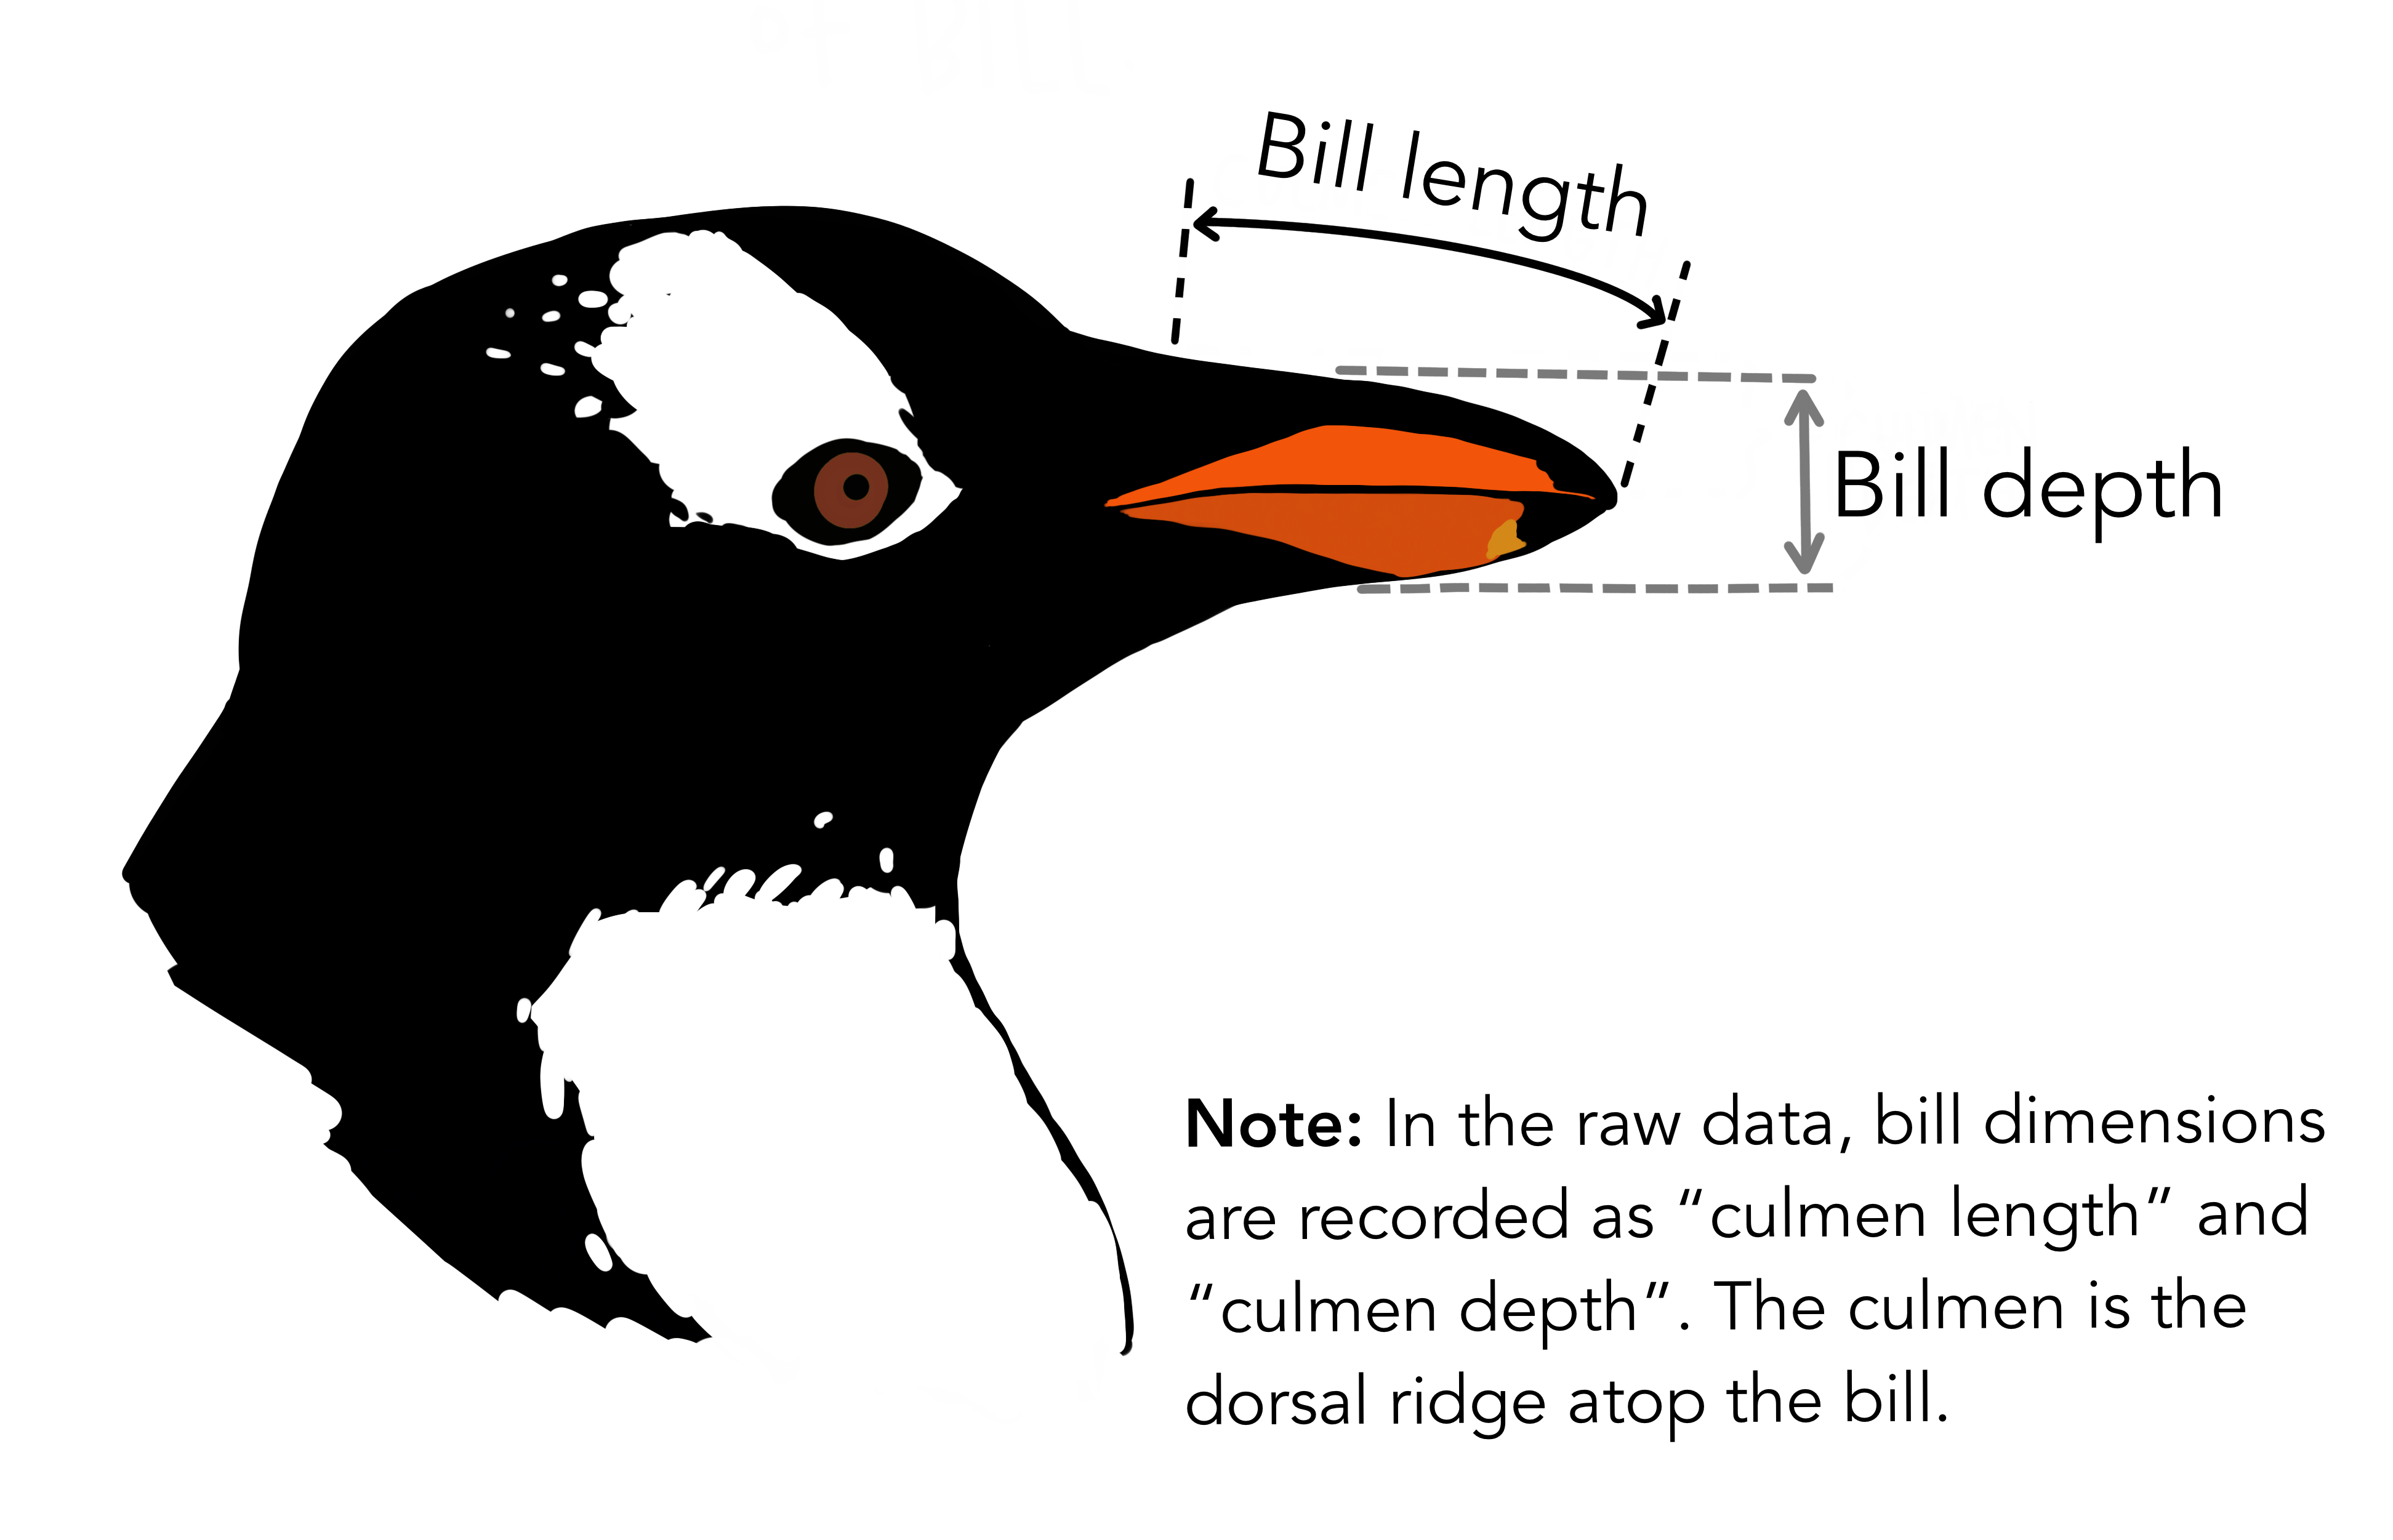
\includegraphics[width=5.44792in,height=\textheight]{https://allisonhorst.github.io/palmerpenguins/reference/figures/culmen_depth.png}
\caption{Diagram of penguin head with indication of bill length and bill
depth.}
\end{figure}

For this \texttt{python} example, I have adapted the code as seen in an
article by
\href{https://towardsdatascience.com/plotly-pandas-for-the-palmer-penguins-f5cdab3c16c8}{Ekta
Sharma} on the Palmer Penguins dataset, go and check it out!

\begin{Shaded}
\begin{Highlighting}[]
\ImportTok{import}\NormalTok{ pandas }\ImportTok{as}\NormalTok{ pd}
\ImportTok{import}\NormalTok{ os}

\CommentTok{\# add the R df into Python}
\NormalTok{penguins\_df }\OperatorTok{=}\NormalTok{ r.penguin\_df}
\end{Highlighting}
\end{Shaded}

\hypertarget{initial-explore}{%
\subsubsection{Initial explore}\label{initial-explore}}

Instead of \texttt{skimr} we can use \texttt{describe()}.

\begin{Shaded}
\begin{Highlighting}[]
\NormalTok{penguins\_df[[}\StringTok{"species"}\NormalTok{, }\StringTok{"sex"}\NormalTok{, }\StringTok{"body\_mass\_g"}\NormalTok{, }\StringTok{"flipper\_length\_mm"}\NormalTok{, }\StringTok{"bill\_length\_mm"}\NormalTok{]].dropna().describe(include}\OperatorTok{=}\StringTok{\textquotesingle{}all\textquotesingle{}}\NormalTok{)}
\end{Highlighting}
\end{Shaded}

\begin{verbatim}
##        species   sex  body_mass_g  flipper_length_mm  bill_length_mm
## count      333   333   333.000000         333.000000      333.000000
## unique       3     2          NaN                NaN             NaN
## top     Adelie  male          NaN                NaN             NaN
## freq       146   168          NaN                NaN             NaN
## mean       NaN   NaN  4207.057057         200.966967       43.992793
## std        NaN   NaN   805.215802          14.015765        5.468668
## min        NaN   NaN  2700.000000         172.000000       32.100000
## 25%        NaN   NaN  3550.000000         190.000000       39.500000
## 50%        NaN   NaN  4050.000000         197.000000       44.500000
## 75%        NaN   NaN  4775.000000         213.000000       48.600000
## max        NaN   NaN  6300.000000         231.000000       59.600000
\end{verbatim}

\begin{center}\rule{0.5\linewidth}{0.5pt}\end{center}

\hypertarget{specific-statistics}{%
\subsubsection{Specific statistics}\label{specific-statistics}}

We can also explore specific statistics

The penguins split by species show a specific relationship between
weight and flipper length, where the Adelie female penguins are the
lighest and have the shortest flippers.

\begin{Shaded}
\begin{Highlighting}[]
\NormalTok{(penguins\_df}
\NormalTok{.dropna()}
\NormalTok{.groupby([}\StringTok{"species"}\NormalTok{, }\StringTok{"sex"}\NormalTok{])}
\NormalTok{.agg(\{}\StringTok{"body\_mass\_g"}\NormalTok{: }\StringTok{"mean"}\NormalTok{, }\StringTok{"flipper\_length\_mm"}\NormalTok{: }\StringTok{"mean"}\NormalTok{, }\StringTok{"sex"}\NormalTok{: }\StringTok{"count"}\NormalTok{\})}
\NormalTok{.sort\_index()}
\NormalTok{)}
\end{Highlighting}
\end{Shaded}

\begin{verbatim}
##                   body_mass_g  flipper_length_mm  sex
## species   sex                                        
## Adelie    female  3368.835616         187.794521   73
##           male    4043.493151         192.410959   73
## Chinstrap female  3527.205882         191.735294   34
##           male    3938.970588         199.911765   34
## Gentoo    female  4679.741379         212.706897   58
##           male    5484.836066         221.540984   61
\end{verbatim}

Looks like the Adelie are the lightest penguin. I want to see their
distribution along with the overall distribution.

\begin{Shaded}
\begin{Highlighting}[]
\NormalTok{smaller }\OperatorTok{=}\NormalTok{ penguins\_df[penguins\_df.species}\OperatorTok{==}\StringTok{"Adelie"}\NormalTok{].dropna()}
\NormalTok{smaller}
\end{Highlighting}
\end{Shaded}

\begin{verbatim}
##     species     island  bill_length_mm  ...  body_mass_g     sex  year
## 0    Adelie  Torgersen            39.1  ...         3750    male  2007
## 1    Adelie  Torgersen            39.5  ...         3800  female  2007
## 2    Adelie  Torgersen            40.3  ...         3250  female  2007
## 4    Adelie  Torgersen            36.7  ...         3450  female  2007
## 5    Adelie  Torgersen            39.3  ...         3650    male  2007
## ..      ...        ...             ...  ...          ...     ...   ...
## 147  Adelie      Dream            36.6  ...         3475  female  2009
## 148  Adelie      Dream            36.0  ...         3450  female  2009
## 149  Adelie      Dream            37.8  ...         3750    male  2009
## 150  Adelie      Dream            36.0  ...         3700  female  2009
## 151  Adelie      Dream            41.5  ...         4000    male  2009
## 
## [146 rows x 8 columns]
\end{verbatim}

\hypertarget{plot-section}{%
\subsubsection{Plot Section}\label{plot-section}}

Let's move on to some plots, for the overall distributions and for just
the Adelie penguins. The overall distribution of the data by species
shows some overlap in body weight for Adelie/Chinstrap, but more of a
separation for the Gentoo penguins.

\begin{Shaded}
\begin{Highlighting}[]
\NormalTok{penguin\_plot }\OtherTok{\textless{}{-}}\NormalTok{ py}\SpecialCharTok{$}\NormalTok{smaller }\SpecialCharTok{\%\textgreater{}\%} 
  \FunctionTok{filter}\NormalTok{(}\SpecialCharTok{!}\FunctionTok{is.na}\NormalTok{(sex)) }\SpecialCharTok{\%\textgreater{}\%} 
  \FunctionTok{ggplot}\NormalTok{(}\FunctionTok{aes}\NormalTok{(body\_mass\_g, }\AttributeTok{fill =}\NormalTok{ sex)) }\SpecialCharTok{+} 
  \FunctionTok{geom\_density}\NormalTok{(}\AttributeTok{color =} \StringTok{"white"}\NormalTok{, }\AttributeTok{alpha =} \FloatTok{0.5}\NormalTok{) }\SpecialCharTok{+}
    \FunctionTok{scale\_fill\_manual}\NormalTok{(}\AttributeTok{values =} \FunctionTok{c}\NormalTok{(}\StringTok{"darkorange"}\NormalTok{,}\StringTok{"purple"}\NormalTok{)) }\SpecialCharTok{+}
  \FunctionTok{labs}\NormalTok{(}\AttributeTok{x =} \StringTok{"Penguin Bins"}\NormalTok{)}

\NormalTok{penguin\_plot}
\end{Highlighting}
\end{Shaded}

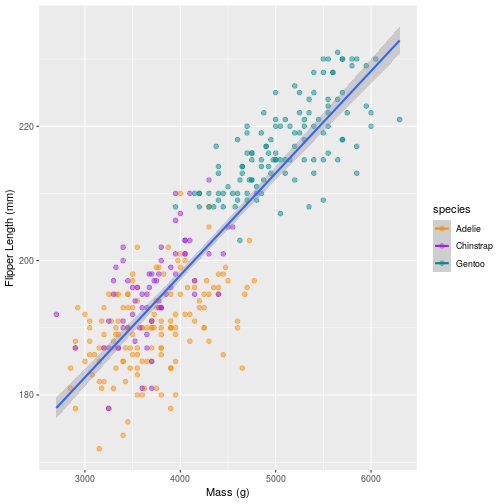
\includegraphics{reticulate-doc_files/figure-latex/unnamed-chunk-5-1.pdf}

\end{document}
